\documentclass[12pt,a4paper]{article}

\usepackage{epcc}
%\usepackage{graphics}
\usepackage{graphicx}
\usepackage{pgfgantt}

% This example file shows how a thesis can be laid out using Latex. It
% does not use any special local features so should be portable to other
% places.
%
% To produce myfile.pdf from myfile.tex type:
% 
% pdflatex myfile
%
% Note that pdflatex expects all included figures to be in PDF too. See
% the includegraphics command below.


% This document contains many cross-references and forward references,
% eg in constructing a table of contents, so Latex may need to be run
% twice to get all the references correct. If you need to run Latex twice
% you may get the warning:
% 
% LaTeX Warning: Label(s) may have changed. Rerun to get cross-references right


\begin{document}

\title{Software Development\\Planning and Risks}
\author{B098688 - s1671778}
\date{\today}

\makeEPCCtitle

\thispagestyle{empty}

\newpage

\pagenumbering{roman}

\tableofcontents


\newpage
\pagenumbering{arabic}

\section{Introduction}

This report will serve as a series of guidelines on how to proceed with the improvement and creation of a web application. The web application has been initiated by an unknown party (very likely the professor of the course), and it must be enhanced such that it fulfills the base requirements for it. A skeleton of the web application that has a few elements already built in. It is, however, very rough and needs much work to become a feasible end product. 

The first part of the report will briefly outline what is the intended project, and the background needed to understand what it is attempting to achieve. While this is being discussed, some of the important factors to keep in mind are highlighted. After this is done, several comments regarding issues in the provided code are made. Afterwards, solutions for most of these are proposed, and eventually presented in a \textit{time/effort} estimation plan. Finally, risk analysis and management strategy are posed.

\section{Project Specifications}

The idea is to further develop a web based application that allows the user to generate a squad for a tabletop game - with certain constraints. The application must allow users to create and edit squads with an unchangeable name, no more than 10 members, and no fewer than 1. The user begins with a Captain, that can become better with time, and has a limited amount of money to hire other regular team members, that cannot improve with time, and a special member, the Ensign, who, like the Captain, can evolve in time.

The idea of the web application is to check that all constraints are fulfilled for a user's squad, and that if one or more are violated, a warning message is displayed such that the user is able to modify their decision. The base stats for each team member are shown in the Annex.

Now, for a new squad the conditions are as follows:

\begin{enumerate}
 \item Squad Name.
 \item Credits: 500 credits.
 \item Captain: \begin{enumerate}
                 \item Only ONE.
                 \item Starts with zero EXPERIENCE.
                 \item Must be assigned some SPECIALISM (Engineering, Psychology, Marksman, Tactics, Melee, Defence).
                 \item ONE Associated Skill must be assigned to the specified SPECIALISM: \begin{enumerate}
							  \item Engineering: [Repair, Sabotage, Augment].
							  \item Psychology: [Bolster, Terror, Counter].
							  \item Marksman: [Aim, Pierce, Reload].
							  \item Tactics: [Squad, Ambush, Surround].
							  \item Melee: [Block, Riposte, Dual].
							  \item Defence: [Shield, Sacrifice, Resolute].
							 \end{enumerate}
				 \item Must be given WEAPONS/EQUIPMENT: \begin{enumerate}
				                                         \item Blaster: 5 credits.
				                                         \item Needle Gun: 12 credits.
				                                         \item Blade: 3 credits.
				                                         \item Cannon: 15 credits.
				                                         \item Whip: 5 credits.
				                                        \end{enumerate}
                \end{enumerate}
 \item Ensign: \begin{enumerate}
                \item Optional: 250 credits.
                \item Maximum ONE.
                \item Must be assigned some SPECIALISM.
                \item Must be assigned some Associated Skill.
                \item Must be given WEAPONS/EQUIPMENT.
               \end{enumerate}
 \item The total number of members is 10 (including the Captain and Ensign).
 \item Prices of hiring are: \begin{enumerate}
                              \item Augment Gorilla: 20 credits.
                              \item Lackey: 20 credits.
                              \item Security: 80 credits.
                              \item Engineer: 60 credits.
                              \item Medic: 50 credits.
                              \item Commando: 100 credits.
                              \item Combat Droid: 150 credits.
                             \end{enumerate}
\end{enumerate}

In order for a new squad to be generated, it must fulfill all the requirements above. 







This report explains a series of performance tests that were made for a 
Predator-Prey model written in Python 3. Said model attempts to describe the 
changes in population densities of hares and pumas over a given landscape. The 
model receives the 
following: a landscape where both animals live together that can contain land 
and water, the population density of each animal, a predation rate (pumas that 
eat hares), birth rates for each animal, mortality rate for pumas (hares do not 
die of natural causes), and diffusion rates for each animal. 

The Predator-Prey model that was analyzed in this report has written by 
\textit{Callum Black, Andr\'es Cathey, and Eskil Joergenssen} for the HPC 
course \textbf{Programming Skills}. This program exploits the resources of the 
python package \texttt{numpy}. Doing so it is able to analyze a $100\%$ 
land-filled 
$2000$x$2000$ landscape in less than $7$ minutes. 

The input file that is given to the program has $0$s and $1$s that represent 
water and land respectively as shown in fig.~\ref{fig:1} (or~\ref{fig:2}) for a 
$30$ by $30$ 
file. When the input file is only water then neither hares nor pumas can live in 
it, and barely no computations should be done. This is the motivation for the 
first performance test that is done for this program, i.e. how is the 
program's run time affected by the land-to-water percentage for a given input 
landscape size, expecting the run time to increase linearly as more land is 
added to a fixed size input landscape.

\begin{figure}[ht]
\begin{minipage}[b]{0.475\linewidth}
\centering
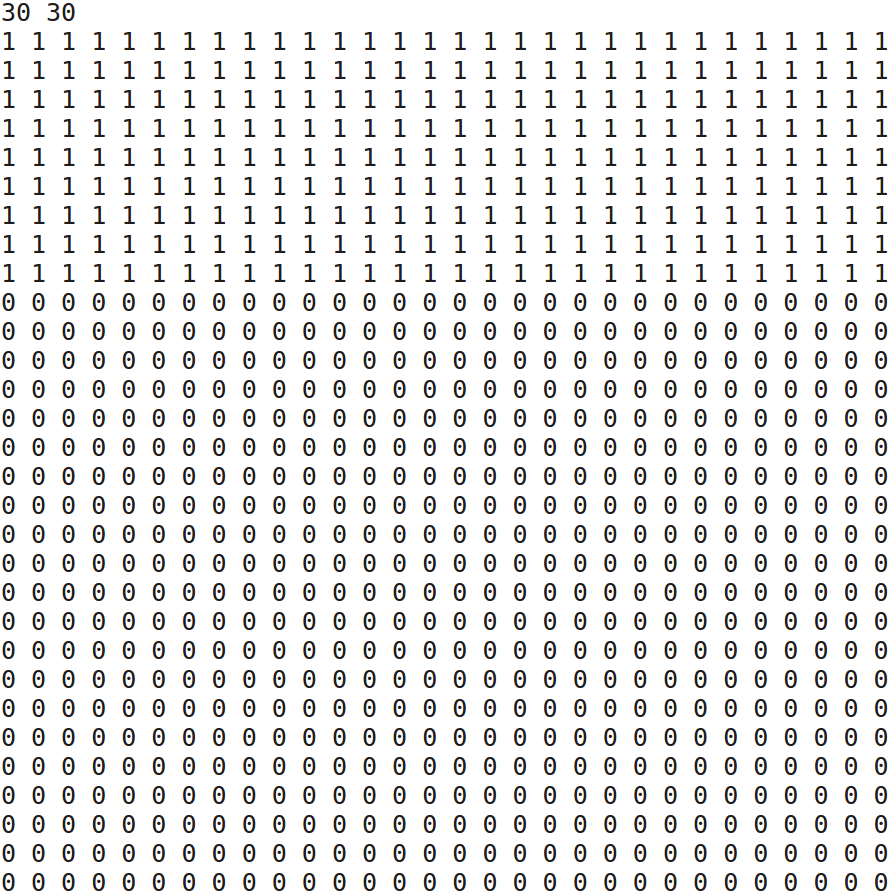
\includegraphics[width=\textwidth]{img/input_file.png}
\caption{An input file with a block of land ($30\%$ land).}
\label{fig:1}
\end{minipage}
\hspace{0.5cm}
\begin{minipage}[b]{0.475\linewidth}
\centering
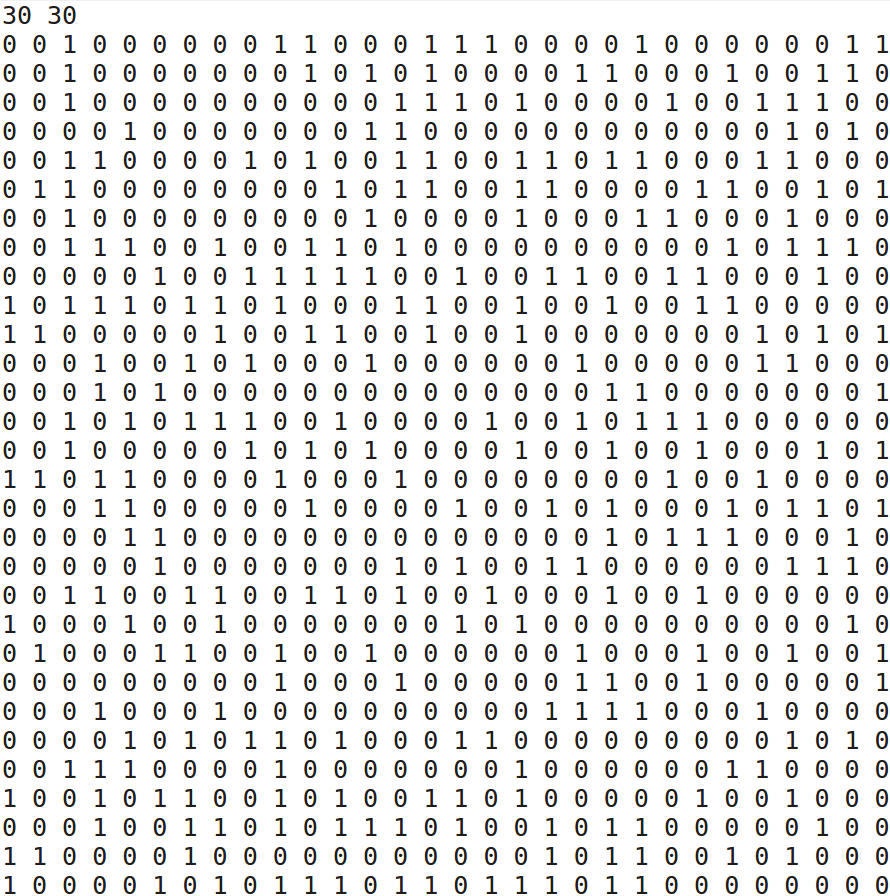
\includegraphics[width=\textwidth]{img/input_rand.png}
\caption{An input file with randomly filled land ($30\%$ land).}
\label{fig:2}
\end{minipage}
\end{figure}

The ``second'' performance test is a slight variation of the first test. It is 
done by taking two different ways of filling the landscape with land. The first 
way to do this is by creating a block of land and a block of water. A different 
way to fill the landscape is to do it in a random manner (without changing the 
percentage of land in the input file) as shown in fig.~\ref{fig:2}. This 
performance test is related to the diffusion rates of both animals (their 
movement within the landscape) - land 
squares in randomized files should, on average, have less land neighbors than 
land squares in 'block' filled files. 

The third test that was done relates to the size of the input file. By changing 
the input landscape area and calculating the run time of the program we expect 
to see a linear growth - failure to observe this would mean that a significant 
optimization in the program. These were done first with a static land 
percentage, and afterwards with varying land-to-water percentages.

Finally, the program was profiled using the python native \texttt{cProfile}. 
This was done for input files of $100$x$100$ and $1000$x$1000$ and, in both 
cases, for $30\%$ and $60\%$ land-to-water ratios. This method was probably the 
most helpful in obtaining information on each function used. It helped 
determine where any optimization attempts should be directed at.

\section{Project Planning}

\newganttchartelement{voidbar}{
    voidbar/.style={
        draw=black,
        top color=black!25,
        bottom color=black!23
    }}
    \begin{ganttchart}[x unit=0.42cm, 
        y unit title=0.7cm,
        y unit chart=0.5cm, vgrid, title label font=\footnotesize,
        canvas/.style={draw=black, dotted}]{1}{28}
        \gantttitle{Hours}{28}\\
        \gantttitlelist{0,5,10,15,20,25,30,35,40,45,50,55,60,65}{2} \\

        \ganttbar{A}{1}{2}     \\ 
        \ganttbar{B}{3}{6}    \\   
        \ganttbar{C}{7}{8}              \\ 
        \ganttbar{D}{9}{12} \\
        \ganttbar{E}{13}{16} \\
        \ganttbar{F}{17}{20} \\
        \ganttbar{G}{7}{8} \\
        \ganttbar{H}{9}{12} \\
        \ganttbar{I}{13}{16} \\
        \ganttbar{J}{16}{21} \\
        \ganttbar{K}{7}{7} \\
        \ganttbar{L}{8}{11} \\
        \ganttbar{M}{12}{14} \\
        \ganttbar{N}{15}{16} \\
        \ganttbar{O}{17}{20} \\
        \ganttbar{P}{21}{24} \\
        \ganttbar{Q}{25}{28} \\
        \ganttbar{R}{28}{28} \\
    \end{ganttchart}

One of the important restrictions of the model is that neither hares nor 
pumas can live in sections that represent water. Therefore it is 
straightforward to expect 
that if a landscape is entirely covered in water it should run faster than one 
completely covered 
in land, since no computations related to the population densities should be 
required. This is the motivation behind the first performance test.

For an input file of fixed size the percentage of land to water is varied from 
$0\%$ to $100\%$. Using a bash script, the time it takes to run the program 
with different land-water proportions in a $100$ by $100$ landscape is plotted 
and fitted to a function as shown in fig.~\ref{fig:3}.

\begin{figure}[ht]
\begin{minipage}[b]{0.475\linewidth}
\centering
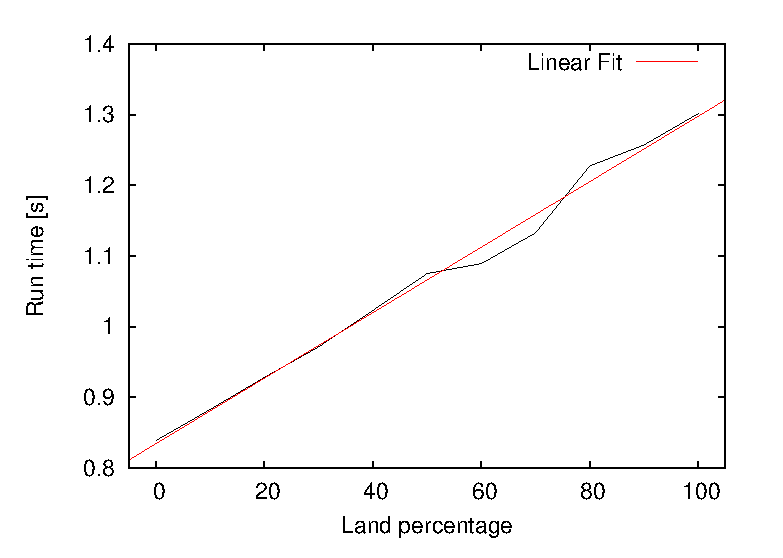
\includegraphics[width=\textwidth]{img/percentage.eps}
\caption{A plot of the run time depending on the percentage of land in the 
'block' input file.}
\label{fig:3}
\end{minipage}
\hspace{0.5cm}
\begin{minipage}[b]{0.475\linewidth}
\centering
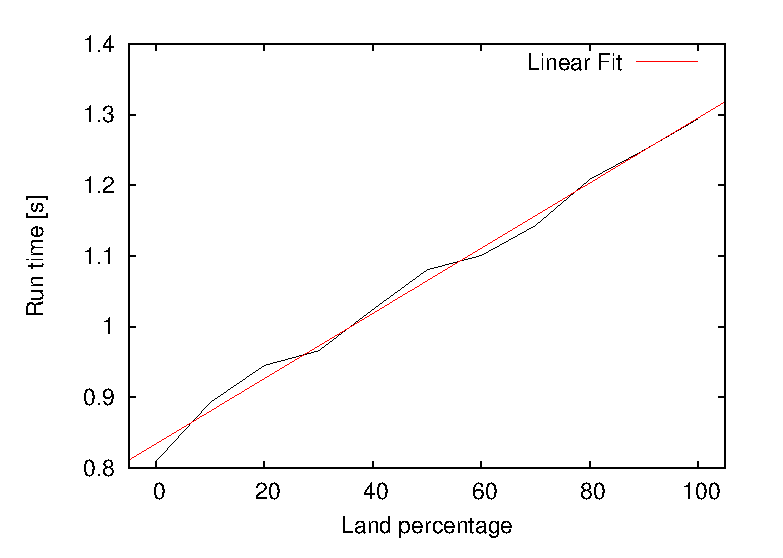
\includegraphics[width=\textwidth]{img/percentage_rand.eps}
\caption{A plot of the run time depending on the percentage of land in the 
random input file.}
\label{fig:4}
\end{minipage}
\end{figure}

The output confirms the intuition that the program's run time should increase 
as the percentage of land in the input landscape file is increased. 
Furthermore, it shows that the aforementioned growth has a direct 
proportionality to the increase in land-to-water ratio, following 
eqn.~\ref{eq:1} 

\begin{equation}
RunTime(land\%)\,=\,0.83451\,+\,0.00463\,land\%
\label{eq:1}
\end{equation}

\subsection{Randomly Generated Landscapes}

The previous performance test was done with ``block'' input landscape files, 
i.e. similar to 
fig.~\ref{fig:1}. The question of whether this would change if the input 
landscape files used were of the likes of fig.~\ref{fig:2} is also briefly 
studied. By doing the exact same analysis as above with randomized land filled 
files gives fig.~\ref{fig:4}, with a fit defined by eqn.~\ref{eq:2}. 

\begin{equation}
RunTime'(land\%)\,=\,0.83434\,+\,0.00461\,land\%
\label{eq:2}
\end{equation}

Since the slope of eqns.~\ref{eq:1} and~\ref{eq:2} define how the computation 
time escalates as the land-to-water percentage increases, a simple comparison 
between the slopes of each equation provides an idea as to whether there is any 
significant difference between both methods. The slope 
of eqn.~\ref{eq:2} differs by less than $1\%$ from the one of eqn.~\ref{eq:1}.
From this it is possible to conclude that it is irrelevant whether the input 
landscape file was randomly generated or generated in a particular order, and 
the factor that needs to be considered is the ratio of land-to-water.

\section{Input Landscape File Size}

The most important aspect of the run time of the program is the size of the 
input landscape file. For the previous performance tests the size of the input 
landscape file was $100$x$100$, which corresponds to a landscape area of 
$10000$. It is of interest to calculate how does the run time behave when we 
linearly increase the landscape area. To do so a bash script is implemented 
that calculates the run time of the program for different landscape areas and 
plots these to check the nature of the growth.

Figure~\ref{fig:5} shows a linear relation between the run time and the input 
landscape's area. Since the input landscapes used are squares, then a quadratic 
relationship between the run time and the input landscape's 
squares per side is expected, and, indeed, observed. This is shown in 
fig.~\ref{fig:6}. Both figures show the run 
time for landscape inputs of land-to-water percentage of $30\%$.

\begin{figure}[ht]
\begin{minipage}[b]{0.475\linewidth}
\centering
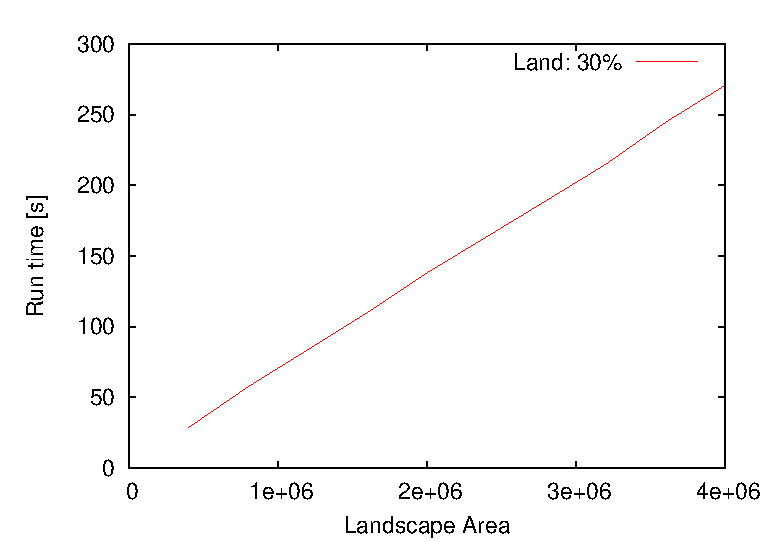
\includegraphics[width=\textwidth]{img/map_size_area_30.eps}
\caption{Run time vs. area with $30\%$ land-to-water.}
\label{fig:5}
\end{minipage}
\hspace{0.5cm}
\begin{minipage}[b]{0.475\linewidth}
\centering
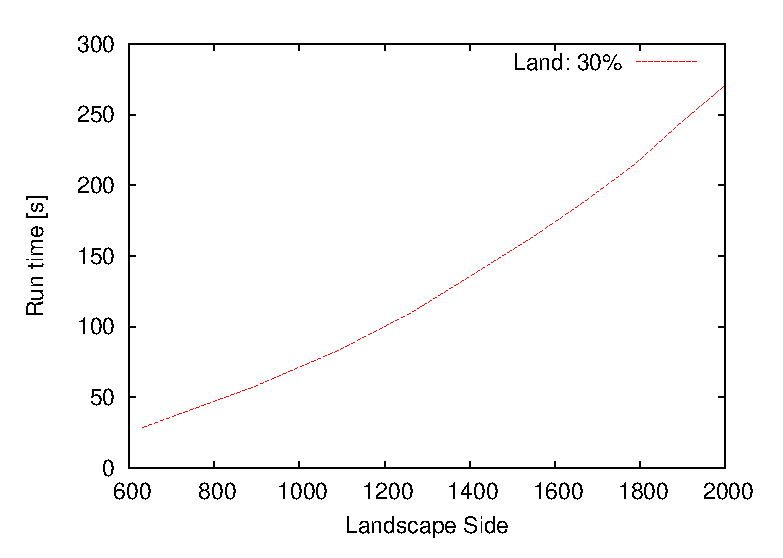
\includegraphics[width=\textwidth]{img/map_size_side_30.eps}
\caption{Run time vs. area with $30\%$ land-to-water.}
\label{fig:6}
\end{minipage}
\end{figure}

To check whether these relations hold for different land-to-water percentages a 
sweep for this is also generated. This is shown in figs.~\ref{fig:7} 
and~\ref{fig:8}. Since the same relation appears for several other 
land-to-water percentages, it is possible to conclude that despite increasing 
the land-to-water percentage in the input file does increase the run time, it 
does so in a linear, and not exponential, fashion. In other words, the run time 
is directly proportional to the landscape area regardless of the land-to-water 
ratio.

\begin{figure}[ht]
\begin{minipage}[b]{0.475\linewidth}
\centering
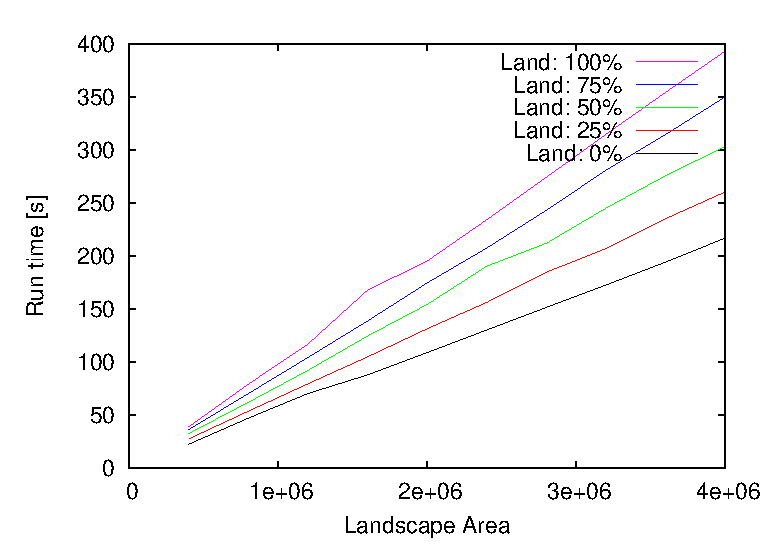
\includegraphics[width=\textwidth]{img/map_size_area.eps}
\caption{Run time vs. area with different land-to-water percentages.}
\label{fig:7}
\end{minipage}
\hspace{0.5cm}
\begin{minipage}[b]{0.475\linewidth}
\centering
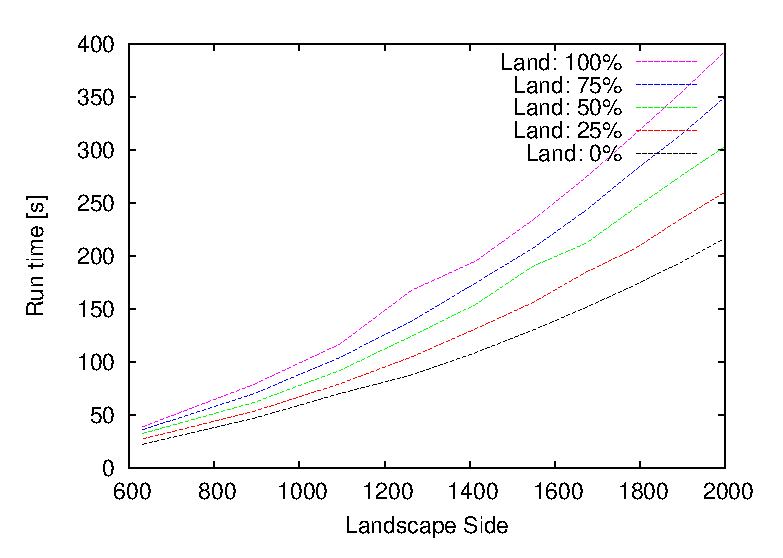
\includegraphics[width=\textwidth]{img/map_size_side.eps}
\caption{Run time vs. area with different land-to-water percentages.}
\label{fig:8}
\end{minipage}
\end{figure}

\section{Code Profiling}

In order to actually know which functions make up for most of the time in the 
run time for the program, the python native profiler ``\texttt{cProfile}'' was 
used. First, two input files of the same size ($100$x$100$) one with $30\%$ and 
the other $60\%$ land-to-water ratios were profiled. The output shows how much 
time each function took and how many times they were called. These results are 
summarized in the pie-charts of figs.~\ref{fig:9} and~\ref{fig:10}.

\begin{figure}[ht]
\begin{minipage}[b]{0.45\linewidth}
\flushleft
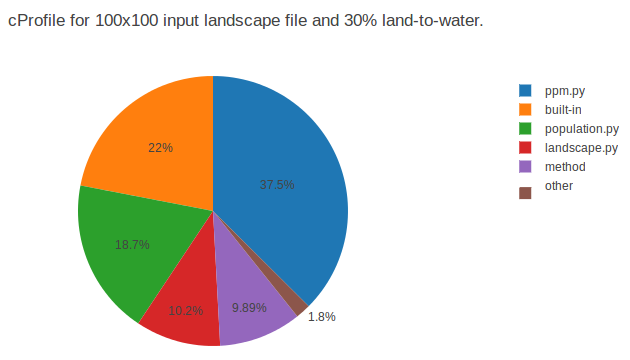
\includegraphics[width=1.1\textwidth]{img/cProfile_30_100.png}
\caption{Pie chart of run time components for $30\%$ 
land-to-water ratio in $100$x$100$ landscape.}
\label{fig:9}
\end{minipage}
\hspace{0.5cm}
\begin{minipage}[b]{0.45\linewidth}
\flushleft
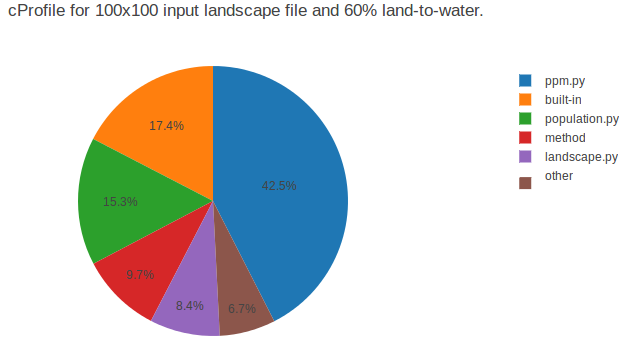
\includegraphics[width=1.1\textwidth]{img/cProfile_60_100.png}
\caption{Pie chart of run time components for $60\%$ 
land-to-water ratio in $100$x$100$ landscape.}
\label{fig:10}
\end{minipage}
\end{figure}

These images show that functions inside the file \texttt{ppm.py} are the 
most time consuming for both the $30\%$ and $60\%$ cases. The 
``\texttt{built-in}'' and ``\texttt{method}'' are instances where 
\texttt{python} 
calls for certain functions, modules, or functions within them. Given that 
the contributions from python calling modules and such will become less 
relevant when larger files are used, we use the ``\texttt{cProfile}'' method 
once more. Obviously, this time the input landscape file will have a larger 
size - $1000$x$1000$. This will help  find out what components of the actual 
program are taking more time.

In this occasion, the landscape input files of $1000$x$1000$ are also 
studied with land-to-water percentages of $30$ and $60$ are used.The 
corresponding pie charts are generated in the same way as before (again with 
a bash script). These are shown figs.~\ref{fig:11} and~\ref{fig:12}.

\begin{figure}[ht]
\begin{minipage}[b]{0.45\linewidth}
\flushleft
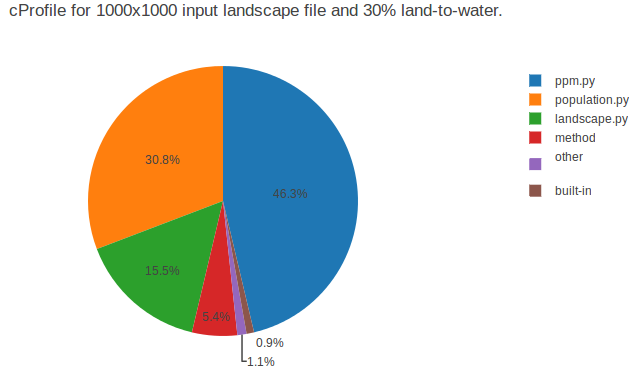
\includegraphics[width=1.1\textwidth]{img/cProfile_30_1000.png}
\caption{Pie chart of run time components for $30\%$ 
land-to-water ratio in $1000$x$1000$ landscape.}
\label{fig:11}
\end{minipage}
\hspace{0.5cm}
\begin{minipage}[b]{0.45\linewidth}
\flushleft
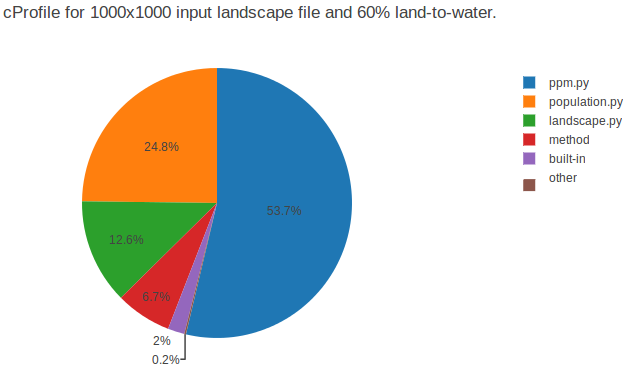
\includegraphics[width=1.1\textwidth]{img/cProfile_60_1000.png}
\caption{Pie chart of run time components for $60\%$ 
land-to-water ratio in $1000$x$1000$ landscape.}
\label{fig:12}
\end{minipage}
\end{figure}

As expected, the pie charts for the larger input file (~\ref{fig:11} and 
~\ref{fig:12}) have a significantly smaller contribution from the 
``\texttt{built-in}'' and ``\texttt{method}'' instances. Additionally, they 
show that the functions of \texttt{ppm.py} are the most time consuming 
regardless of the land-to-water percentage and the input file size.

These figures provide a more complete picture of what can be done to optimize 
the program under study. The first thing that is evident is that 
\texttt{ppm.py} is using most of the run time in all four cases. This file 
holds the functions that are used to generate the \texttt{.ppm} files. Hence 
this is where it would be most beneficial to attempt some type of 
optimization. Additionally, the second set of pie charts makes it clear that 
the files \texttt{population.py} and \texttt{landscape.py} are also good 
candidates for possible optimization.


\section{Conclusions}

After performing a series of performance and profiling tests on the program 
written by \textit{Callum Black, Andr\'es Cathey, and Eskil Joergenssen} for the 
HPC course \textbf{Programming Skills} a few good features can be made 
about the 
run times of said program. Additionally, it was possible to know what functions 
should be optimized in order to do a significant impact on the program's run 
time.

The first feature of the code that was studied was how the program's run time 
increases as the land-to-water percentage is increased. A linear relation 
between these was found, confirming that the computation time increases when 
the percentage of land in a fixed size file is increased. 

Afterwards, it was shown that the program's run time also grows linearly when 
the input landscape file's number of land/water squares is increased linearly. 
This confirmed the intuition that the most important factor for the program's 
run time is the landscape's area. 

Finally, the profiling part of the tests provided information as to what 
functions could be optimized in order to decrease the run-time of the program. 
Said optimizations should be done for writing the \texttt{.ppm} file, since 
this always represents most of the run time regardless of input file size (the 
percentage of the run time that it represents should also grow linearly).

It can be concluded that performance testing and profiling are important to 
know what are the weaknesses and the strengths of large, or complex, codes that 
cannot be studied by simply going through them. These methods are also very 
useful to know what sections of a code is taking up most of the run time and, 
thus, best suited for optimization.



%\begin{table}[h]
%\begin{center}
%\begin{tabular}{||l|c|l||}
%\hline
%{\bf File names} & {\bf Satellite} & {\bf Resolution}\\
%\hline
%  worldr         &  Meteosat     &   5km\\
%  worldg         &  Meteosat     &   5km\\
%  worldb         &  Meteosat     &   5km\\
%\hline
%\end{tabular}
%\end{center}
%\caption{This is a simple table. More complicated tables can have
%headings which pass over more than one column}
%\label{simple_table}
%\end{table}



%\begin{thebibliography}{100}

%\bibitem{ref:lam} L.Lamport. {\em 1986 Latex User's Guide
%and Reference Manual.} Addison Wesley. pp242.

%\bibitem{ref:bloggs} F.Bloggs. {\em 1993 Latex Users do it
%in Environments} Int. Journal of Silly Findings. pp 23-29.

%\end{thebibliography}


\end{document}

